\upaper{0}{Foreword}
\author{Divine Counsellor}
\vs p000 0:1 In the minds of the mortals of Urantia --- that being the name of your world\fnst{\textbf{Urantia}, pronounced \textit{oor\'antia}, is a coined word from the Greek \textgreek{οὐρανός} ``heavens'' and the Latin suffix \textit{-tia}, probably signifying ``[y]our place in the heavens''.} --- there exists great confusion respecting the meaning of such terms as God, divinity, and deity. Human beings are still more confused and uncertain about the relationships of the divine personalities designated by these numerous appellations. Because of this conceptual poverty associated with so much ideational confusion, I have been directed to formulate this introductory statement in explanation of the meanings which should be attached to certain word symbols as they may be hereinafter used in those papers which the Orvonton\fnst{\textbf{Orvonton}, is a coined word from the Old English prefix \textit{or-} ``out'', the Middle English \textit{wone} (> \textit{von}) ``dwelling place'' and the Old English \textit{tun} ``town'', resulting in the total meaning of ``the out-dwelling town''.} corps of truth revealers have been authorized\fnst{\textbf{Orvonton \ldots\ authorized}, Only the papers 1--31 (i.e. Part I) were authorized at the superuniverse level. The papers 32--196 (Parts II, III and IV) were revealed under the local universe and system level authorization.} to translate into the English language of Urantia\fnst{\textbf{the English language of Urantia}, See \bibref[82:6.5]{p082 6:5} for a possible explanation why this language was chosen.}.
\vs p000 0:2 It is exceedingly difficult to present enlarged concepts and advanced truth, in our endeavour to expand cosmic consciousness and enhance spiritual perception, when we are restricted to the use of a circumscribed language of the realm. But our mandate admonishes us to make every effort to convey our meanings by using the word symbols of the English tongue. We have been instructed to introduce new terms only when the concept to be portrayed finds no terminology in English which can be employed to convey such a new concept partially or even with more or less distortion of meaning.
\vs p000 0:3 In the hope of facilitating comprehension and of preventing confusion on the part of every mortal who may peruse these papers, we deem it wise to present in this initial statement an outline of the meanings to be attached to numerous English words which are to be employed in designation of Deity and certain associated concepts of the things, meanings, and values of universal reality.
\vs p000 0:4 But in order to formulate this Foreword of definitions and limitations of terminology, it is necessary to anticipate the usage of these terms in the subsequent presentations. This Foreword is not, therefore, a finished statement within itself; it is only a definitive guide designed to assist those who shall read the accompanying papers dealing with Deity and the universe of universes\fnst{\textbf{papers dealing with Deity and the universe of universes}, As already noted at \bibref[0:0.1]{p000 0:1} these are limited to papers 1--31 only. Therefore, this Foreword is properly ``the Foreword to Part I of the Urantia Papers'' and that is where it should be printed. Curiously, this is where the Foreword is found in ``The Titles of the Papers'' and ``Contents of the Book'' as printed in the original 1955 edition, although the text of the Foreword is printed just before the Part I title page preceding Paper 1 of that edition. Moving the Foreword outside Part I (as is done in all editions except the present one) shows an attempt to \bibemph{fossilize} into a single monolithic ``Urantia \textbf{Book}'' what should remain a living and constantly growing set of ``Urantia \textbf{Papers}'' --- an epochal revelation of the living God to growing evolving mortals.} which have been formulated by an Orvonton commission sent to Urantia for this purpose.
\vs p000 0:5 \pc Your world, Urantia, is one of many similar inhabited planets which comprise the local universe of \bibemph{Nebadon}\fnst{\textbf{\bibemph{Nebadon}}, is a coined word from the Old English \textit{adune} (> \textit{dune} > \textit{dun} > \textit{don}) ``off the hill'', resulting in the probable total meaning of ``the nebular hill''. Indeed, the Nebadon (local universe) level of our ascension is a relative `hill', compared to the system-level mansion world experience.}. This universe, together with similar creations, makes up the superuniverse of \bibemph{Orvonton,} from whose capital, Uversa\fnst{\textbf{Uversa}, is a coined word from the Latin \textit{versatilis} ``capable of turning or being turned around'', signifying the centre of the superuniverse expressing the 7\ts{th} expression of the Father-Son-Spirit pattern: `U' being the 21\ts{st} letter of English alphabet: $21=3\times 7$. The name of the capital of the first evolutionary superuniverse, under this scheme, would be ``Cversa'', of the second --- ``Fversa'', and so on.}, our commission hails. Orvonton is one of the seven evolutionary superuniverses of time and space which circle the never\hyp{}beginning, never\hyp{}ending creation of divine perfection --- the central universe of \bibemph{Havona.} At the heart of this eternal and central universe is the stationary Isle of Paradise, the geographic centre of infinity and the dwelling place of the eternal God.
\vs p000 0:6 The seven evolving superuniverses in association with the central and divine universe, we commonly refer to as the \bibemph{grand universe;} these are the now organized and inhabited creations. They are all a part of the \bibemph{master universe,} which also embraces the uninhabited but mobilizing universes of outer space.
\usection{1.\bibnobreakspace Deity and Divinity}
\vs p000 1:1 The universe of universes presents phenomena of deity activities on diverse levels of cosmic realities, mind meanings, and spirit values, but all of these ministrations --- personal or otherwise --- are divinely co\hyp{}ordinated.
\vs p000 1:2 \pc DEITY is personalizable as God, is prepersonal and superpersonal in ways not altogether comprehensible by man. Deity is characterized by the quality of unity --- actual or potential --- on all supermaterial levels of reality; and this unifying quality is best comprehended by creatures as divinity.
\vs p000 1:3 \pc Deity functions on personal, prepersonal, and superpersonal levels. Total Deity is functional on the following seven levels:
\vs p000 1:4 \ublistelem{1.}\bibnobreakspace \bibemph{Static ---} self\hyp{}contained and self\hyp{}existent Deity.
\vs p000 1:5 \ublistelem{2.}\bibnobreakspace \bibemph{Potential ---} self\hyp{}willed and self\hyp{}purposive Deity.
\vs p000 1:6 \ublistelem{3.}\bibnobreakspace \bibemph{Associative ---} self\hyp{}personalized and divinely fraternal Deity.
\vs p000 1:7 \ublistelem{4.}\bibnobreakspace \bibemph{Creative ---} self\hyp{}distributive and divinely revealed Deity.
\vs p000 1:8 \ublistelem{5.}\bibnobreakspace \bibemph{Evolutional ---} self\hyp{}expansive and creature\hyp{}identified Deity.
\vs p000 1:9 \ublistelem{6.}\bibnobreakspace \bibemph{Supreme ---} self\hyp{}experiential and creature\hyp{}Creator\hyp{}unifying Deity. Deity functioning on the first creature\hyp{}identificational level as time\hyp{}space overcontrollers of the grand universe, sometimes designated the Supremacy of Deity.
\vs p000 1:10 \ublistelem{7.}\bibnobreakspace \bibemph{Ultimate ---} self\hyp{}projected and time\hyp{}space\hyp{}transcending Deity. Deity omnipotent, omniscient, and omnipresent. Deity functioning on the second level of unifying divinity expression as effective overcontrollers and absonite upholders of the master universe. As compared with the ministry of the Deities to the grand universe, this absonite function in the master universe is tantamount to universal overcontrol and supersustenance, sometimes called the Ultimacy of Deity.
\vs p000 1:11 \pc \bibemph{The finite level} of reality is characterized by creature life and time\hyp{}space limitations. Finite realities may not have endings, but they always have beginnings --- they are created. The Deity level of Supremacy may be conceived as a function in relation to finite existences.
\vs p000 1:12 \pc \bibemph{The absonite level} of reality is characterized by things and beings without beginnings or endings and by the transcendence of time and space. Absoniters are not created; they are eventuated --- they simply are. The Deity level of Ultimacy connotes a function in relation to absonite realities. No matter in what part of the master universe, whenever time and space are transcended, such an absonite phenomenon is an act of the Ultimacy of Deity.
\vs p000 1:13 \pc \bibemph{The absolute level} is beginningless, endless, timeless, and spaceless. For example: On Paradise, time and space are nonexistent; the time\hyp{}space status of Paradise is absolute. This level is Trinity attained, existentially, by the Paradise Deities, but this third level of unifying Deity expression is not fully unified experientially. Whenever, wherever, and however the absolute level of Deity functions, Paradise\hyp{}absolute values and meanings are manifest.
\vs p000 1:14 \pc Deity may be existential\fnst{\textbf{existential}, Defined at \bibref[0:7.3]{p000 7:3} as ``beings of eternal existence, past, present, and future''.}, as in the Eternal Son; experiential\fnst{\textbf{experiential}, Defined at \bibref[0:7.4]{p000 7:4} as ``beings actualizing in the post\hyp{}Havona present but of unending existence throughout all future eternity''.}, as in the Supreme Being; associative, as in God the Sevenfold; undivided, as in the Paradise Trinity.
\vs p000 1:15 Deity is the source of all that which is divine. Deity is characteristically and invariably divine, but all that which is divine is not necessarily Deity, though it will be co\hyp{}ordinated with Deity and will tend towards some phase of unity with Deity --- spiritual, mindal, or personal.
\vs p000 1:16 \pc DIVINITY is the characteristic, unifying, and co\hyp{}ordinating quality of Deity.
\vs p000 1:17 Divinity is creature comprehensible as truth, beauty, and goodness; correlated in personality as love, mercy, and ministry; disclosed on impersonal levels as justice, power, and sovereignty.
\vs p000 1:18 Divinity may be perfect --- complete --- as on existential and creator levels of Paradise perfection; it may be imperfect, as on experiential and creature levels of time\hyp{}space evolution; or it may be relative, neither perfect nor imperfect, as on certain Havona levels of existential\hyp{}experiential relationships.
\vs p000 1:19 \pc When we attempt to conceive of perfection in all phases and forms of relativity, we encounter seven conceivable types\fnst{\textbf{seven conceivable types}, The following list of seven elements contains all non-empty subsets ($2^3 - 1 = 7$) of the set \{Absolute, Relative, Imperfection\}, listed in this particular order to reflect the inherent ordering of the three basic elements as follows: Absolute > Relative > Imperfection.}:
\vs p000 1:20 \ublistelem{1.}\bibnobreakspace Absolute perfection in all aspects.
\vs p000 1:21 \ublistelem{2.}\bibnobreakspace Absolute perfection in some phases and relative perfection in all other aspects.
\vs p000 1:22 \ublistelem{3.}\bibnobreakspace Absolute, relative, and imperfect aspects in varied association.
\vs p000 1:23 \ublistelem{4.}\bibnobreakspace Absolute perfection in some respects, imperfection in all others.
\vs p000 1:24 \ublistelem{5.}\bibnobreakspace Absolute perfection in no direction, relative perfection in all\fnc{\textbf{all}, In 1955 text: all other.} manifestations.
\vs p000 1:25 \ublistelem{6.}\bibnobreakspace Absolute perfection in no phase, relative in some, imperfect in others.
\vs p000 1:26 \ublistelem{7.}\bibnobreakspace Absolute perfection in no attribute, imperfection in all.
\usection{2.\bibnobreakspace God}
\vs p000 2:1 Evolving mortal creatures experience an irresistible urge to symbolize their finite concepts of God. Man’s consciousness of moral duty and his spiritual idealism represent a value level --- an experiential reality --- which is difficult of symbolization.
\vs p000 2:2 Cosmic consciousness implies the recognition of a First Cause, the one and only uncaused reality. God, the Universal Father, functions on three Deity\hyp{}personality levels of subinfinite value and relative divinity expression:
\vs p000 2:3 \ublistelem{1.}\bibnobreakspace \bibemph{Prepersonal ---} as in the ministry of the Father fragments, such as the Thought Adjusters.
\vs p000 2:4 \ublistelem{2.}\bibnobreakspace \bibemph{Personal ---} as in the evolutionary experience of created and procreated beings.
\vs p000 2:5 \ublistelem{3.}\bibnobreakspace \bibemph{Superpersonal ---} as in the eventuated existences of certain absonite and associated beings.
\vs p000 2:6 GOD is a word symbol designating all personalizations of Deity. The term requires a different definition on each personal level of Deity function and must be still further redefined within each of these levels, as this term may be used to designate the diverse co\hyp{}ordinate and subordinate personalizations of Deity; for example: the Paradise Creator Sons --- the local universe fathers.
\vs p000 2:7 \pc The term God, as we make use of it, may be understood:
\vs p000 2:8 \bibemph{By designation ---} as God the Father.
\vs p000 2:9 \bibemph{By context ---} as when used in the discussion of some one deity level or association. When in doubt as to the exact interpretation of the word God, it would be advisable to refer it to the person of the Universal Father.
\vs p000 2:10 \pc The term God always denotes \bibemph{personality.} Deity may, or may not, refer to divinity personalities.
\vs p000 2:11 \pc The word GOD is used, in these papers, with the following meanings:
\vs p000 2:12 \ublistelem{1.}\bibnobreakspace \bibemph{God the Father ---} Creator, Controller, and Upholder. The Universal Father, the First Person of Deity.
\vs p000 2:13 \ublistelem{2.}\bibnobreakspace \bibemph{God the Son ---} Co\hyp{}ordinate Creator, Spirit Controller, and Spiritual Administrator. The Eternal Son, the Second Person of Deity.
\vs p000 2:14 \ublistelem{3.}\bibnobreakspace \bibemph{God the Spirit ---} Conjoint Actor, Universal Integrator, and Mind Bestower. The Infinite Spirit, the Third Person of Deity.
\vs p000 2:15 \ublistelem{4.}\bibnobreakspace \bibemph{God the Supreme ---} the actualizing or evolving God of time and space. Personal Deity associatively realizing the time\hyp{}space experiential achievement of creature\hyp{}Creator identity. The Supreme Being is personally experiencing the achievement of Deity unity as the evolving and experiential God of the evolutionary creatures of time and space.
\vs p000 2:16 \ublistelem{5.}\bibnobreakspace \bibemph{God the Sevenfold ---} Deity personality anywhere actually functioning in time and space. The personal Paradise Deities and their creative associates functioning in and beyond the borders of the central universe and power\hyp{}personalizing as the Supreme Being on the first creature level of unifying Deity revelation in time and space. This level, the grand universe, is the sphere of the time\hyp{}space descension of Paradise personalities in reciprocal association with the time\hyp{}space ascension of evolutionary creatures.
\vs p000 2:17 \ublistelem{6.}\bibnobreakspace \bibemph{God the Ultimate ---} the eventuating God of supertime and transcended space. The second experiential level of unifying Deity manifestation. God the Ultimate implies the attained realization of the synthesized absonite\hyp{}superpersonal, time\hyp{}space\hyp{}transcended, and eventuated\hyp{}experiential values, co\hyp{}ordinated on final creative levels of Deity reality.
\vs p000 2:18 \ublistelem{7.}\bibnobreakspace \bibemph{God the Absolute ---} the experientializing God of transcended superpersonal values and divinity meanings, now existential as the \bibemph{Deity Absolute.} This is the third level of unifying Deity expression and expansion. On this supercreative level, Deity experiences exhaustion of personalizable potential, encounters completion of divinity, and undergoes depletion of capacity for self\hyp{}revelation to successive and progressive levels of other\hyp{}personalization. Deity now encounters, impinges upon, and experiences identity with, the \bibemph{Unqualified Absolute.}
\usection{3.\bibnobreakspace The First Source and Centre}
\vs p000 3:1 Total, infinite reality is existential in seven phases and as seven co\hyp{}ordinate Absolutes:
\vs p000 3:2 \ublistelem{1.}\bibnobreakspace The First Source and Centre.
\vs p000 3:3 \ublistelem{2.}\bibnobreakspace The Second Source and Centre.
\vs p000 3:4 \ublistelem{3.}\bibnobreakspace The Third Source and Centre.
\vs p000 3:5 \ublistelem{4.}\bibnobreakspace The Isle of Paradise.
\vs p000 3:6 \ublistelem{5.}\bibnobreakspace The Deity Absolute.
\vs p000 3:7 \ublistelem{6.}\bibnobreakspace The Universal Absolute.
\vs p000 3:8 \ublistelem{7.}\bibnobreakspace The Unqualified Absolute.
\vs p000 3:9 \pc God, as the First Source and Centre, is primal in relation to total reality --- unqualifiedly. The First Source and Centre is infinite as well as eternal and is therefore limited or conditioned only by volition.\tunemarkup{pictures}{\begin{figure}[H]\centering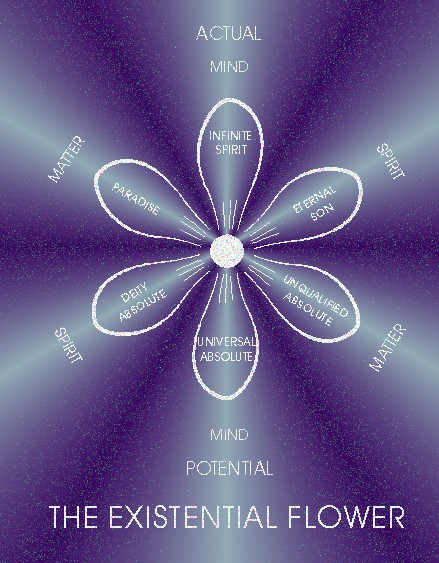
\includegraphics[scale=\tunemarkup{pgkoboaurahd}{0.6}\tunemarkup{pghanlin}{0.52}\tunemarkup{pgnexus7}{0.56}\tunemarkup{pgkindledx}{0.43}]{images/Existential-Flower.jpg}\caption{The Existential Flower by Troy~R.~Bishop}\end{figure}}
\vs p000 3:10 God --- the Universal Father --- is the personality of the First Source and Centre and as such maintains personal relations of infinite control over all co\hyp{}ordinate and subordinate sources and centres. Such control is personal and infinite in \bibemph{potential,} even though it may never actually function owing to the perfection of the function of such co\hyp{}ordinate and subordinate sources and centres and personalities.
\vs p000 3:11 The First Source and Centre is, therefore, primal in all domains: deified or undeified, personal or impersonal, actual or potential, finite or infinite. No thing or being, no relativity or finality, exists except in direct or indirect relation to, and dependence on, the primacy of the First Source and Centre.
\vs p000 3:12 \pc \bibemph{The First Source and Centre} is related to the universe as:
\vs p000 3:13 \ublistelem{1.}\bibnobreakspace The gravity forces of the material universes are convergent in the gravity centre of nether Paradise. That is just why the geographic location of his person is eternally fixed in absolute relation to the force\hyp{}energy centre of the nether or material plane of Paradise. But the absolute personality of Deity exists on the upper or spiritual plane of Paradise.
\vs p000 3:14 \ublistelem{2.}\bibnobreakspace The mind forces are convergent in the Infinite Spirit; the differential and divergent cosmic mind in the Seven Master Spirits; the factualizing mind of the Supreme as a time\hyp{}space experience in Majeston.
\vs p000 3:15 \ublistelem{3.}\bibnobreakspace The universe spirit forces are convergent in the Eternal Son.
\vs p000 3:16 \ublistelem{4.}\bibnobreakspace The unlimited capacity for deity action resides in the Deity Absolute.
\vs p000 3:17 \ublistelem{5.}\bibnobreakspace The unlimited capacity for infinity response exists in the Unqualified Absolute.
\vs p000 3:18 \ublistelem{6.}\bibnobreakspace The two Absolutes --- Qualified and Unqualified --- are co\hyp{}ordinated and unified in and by the Universal Absolute.
\vs p000 3:19 \ublistelem{7.}\bibnobreakspace The potential personality of an evolutionary moral being or of any other moral being is centred in the personality of the Universal Father.
\vs p000 3:20 \pc REALITY, as comprehended by finite beings, is partial, relative, and shadowy. The maximum Deity reality fully comprehensible by evolutionary finite creatures is embraced within the Supreme Being. Nevertheless there are antecedent and eternal realities, superfinite realities, which are ancestral to this Supreme Deity of evolutionary time\hyp{}space creatures. In attempting to portray the origin and nature of universal reality, we are forced to employ the technique of time\hyp{}space reasoning in order to reach the level of the finite mind. Therefore must many of the simultaneous events of eternity be presented as sequential transactions.
\vs p000 3:21 As a time\hyp{}space creature would view the origin and differentiation of Reality, the eternal and infinite I AM achieved Deity liberation from the fetters of unqualified infinity through the exercise of inherent and eternal free will, and this divorcement from unqualified infinity produced the first \bibemph{absolute divinity\hyp{}tension.} This tension of infinity differential is resolved by the Universal Absolute, which functions to unify and co\hyp{}ordinate the dynamic infinity of Total Deity and the static infinity of the Unqualified Absolute.
\vs p000 3:22 In this original transaction the theoretical I AM achieved the realization of personality by becoming the Eternal Father of the Original Son simultaneously with becoming the Eternal Source of the Isle of Paradise. Coexistent with the differentiation of the Son from the Father, and in the presence of Paradise, there appeared the person of the Infinite Spirit and the central universe of Havona. With the appearance of coexistent personal Deity, the Eternal Son and the Infinite Spirit, the Father escaped, as a personality, from otherwise inevitable diffusion throughout the potential of Total Deity. Thenceforth it is only in Trinity association with his two Deity equals that the Father fills all Deity potential, while increasingly experiential Deity is being actualized on the divinity levels of Supremacy, Ultimacy, and Absoluteness.
\vs p000 3:23 \pc \bibemph{The concept of the I AM} is a philosophic concession which we make to the time\hyp{}bound, space\hyp{}fettered, finite mind of man, to the impossibility of creature comprehension of eternity existences --- nonbeginning, nonending realities and relationships. To the time\hyp{}space creature, all things must have a beginning save only the ONE UNCAUSED --- the primeval cause of causes. Therefore do we conceptualize this philosophic value\hyp{}level as the I AM, at the same time instructing all creatures that the Eternal Son and the Infinite Spirit are coeternal with the I AM; in other words, that there never was a time when the I AM was not the \bibemph{Father} of the Son and, with him, of the Spirit.
\vs p000 3:24 \pc \bibemph{The Infinite} is used to denote the fullness --- the finality --- implied by the primacy of the First Source and Centre. The \bibemph{theoretical} I AM is a creature\hyp{}philosophic extension of the “infinity of will,” but the Infinite is an \bibemph{actual} value\hyp{}level representing the eternity\hyp{}intension of the true infinity of the absolute and unfettered free will of the Universal Father. This concept is sometimes designated the Father\hyp{}Infinite.
\vs p000 3:25 Much of the confusion of all orders of beings, high and low, in their efforts to discover the Father\hyp{}Infinite, is inherent in their limitations of comprehension. The absolute primacy of the Universal Father is not apparent on subinfinite levels; therefore is it probable that only the Eternal Son and the Infinite Spirit truly know the Father as an infinity; to all other personalities such a concept represents the exercise of faith.
\usection{4.\bibnobreakspace Universe Reality}
\vs p000 4:1 Reality differentially actualizes on diverse universe levels; reality originates in and by the infinite volition of the Universal Father and is realizable in three primal phases on many different levels of universe actualization:
\vs p000 4:2 \ublistelem{1.}\bibnobreakspace \bibemph{Undeified reality} ranges from the energy domains of the nonpersonal to the reality realms of the nonpersonalizable values of universal existence, even to the presence of the Unqualified Absolute.
\vs p000 4:3 \ublistelem{2.}\bibnobreakspace \bibemph{Deified reality} embraces all\fnc{\textbf{all}, In 1955 text: all of. \bibexpl{The committee decided that this revised phraseology is all-inclusive without implying any limitations and without requiring a change of tone.}} infinite Deity potentials ranging upward through all realms of personality from the lowest finite to the highest infinite, thus encompassing the domain of all that which is personalizable and more --- even to the presence of the Deity Absolute.
\vs p000 4:4 \ublistelem{3.}\bibnobreakspace \bibemph{Interassociated reality.} Universe reality is supposedly either deified or undeified, but to subdeified beings there exists a vast domain of interassociated reality, potential and actualizing, which is difficult of identification. Much of this co\hyp{}ordinate reality is embraced within the realms of the Universal Absolute.
\vs p000 4:5 This is the primal concept of original reality: The Father initiates and maintains Reality. The primal \bibemph{differentials} of reality are the deified and the undeified --- the Deity Absolute and the Unqualified Absolute. The primal \bibemph{relationship} is the tension between them. This Father\hyp{}initiated divinity\hyp{}tension is perfectly resolved by, and eternalizes as, the Universal Absolute.
\vs p000 4:6 \pc From the viewpoint of time and space, reality is further divisible as:
\vs p000 4:7 \ublistelem{1.}\bibnobreakspace \bibemph{Actual and Potential.} Realities existing in fullness of expression in contrast to those which carry undisclosed capacity for growth. The Eternal Son is an absolute spiritual actuality; mortal man is very largely an unrealized spiritual potentiality.
\vs p000 4:8 \ublistelem{2.}\bibnobreakspace \bibemph{Absolute and Subabsolute.} Absolute realities are eternity existences. Subabsolute realities are projected on two levels: Absonites --- realities which are relative with respect to both time and eternity. Finites --- realities which are projected in space and are actualized in time.
\vs p000 4:9 \ublistelem{3.}\bibnobreakspace \bibemph{Existential and Experiential.} Paradise Deity is existential, but the emerging Supreme and Ultimate are experiential.
\vs p000 4:10 \ublistelem{4.}\bibnobreakspace \bibemph{Personal and Impersonal.} Deity expansion, personality expression, and universe evolution are forever conditioned by the Father’s freewill act which forever separated the mind\hyp{}spirit\hyp{}personal meanings and values of actuality and potentiality centring in the Eternal Son from those things which centre and inhere in the eternal Isle of Paradise.
\vs p000 4:11 \pc PARADISE is a term inclusive of the personal and the nonpersonal focal Absolutes of all phases of universe reality. Paradise, properly qualified, may connote any and all forms of reality, Deity, divinity, personality, and energy --- spiritual, mindal, or material. All share Paradise as the place of origin, function, and destiny, as regards values, meanings, and factual existence.
\vs p000 4:12 \pc \bibemph{The Isle of Paradise ---} Paradise not otherwise qualified --- is the Absolute of the material\hyp{}gravity control of the First Source and Centre. Paradise is motionless, being the only stationary thing in the universe of universes. The Isle of Paradise has a universe location but no position in space. This eternal Isle is the actual source of the physical universes --- past, present, and future. The nuclear Isle of Light is a Deity derivative, but it is hardly Deity; neither are the material creations a part of Deity; they are a consequence.
\vs p000 4:13 Paradise is not a creator; it is a unique controller of many universe activities, far more of a controller than a reactor. Throughout the material universes Paradise influences the reactions and conduct of all beings having to do with force, energy, and power, but Paradise itself is unique, exclusive, and isolated in the universes. Paradise represents nothing and nothing represents Paradise. It is neither a force nor a presence; it is just \bibemph{Paradise.}
\usection{5.\bibnobreakspace Personality Realities}
\vs p000 5:1 Personality is a level of deified reality and ranges from the mortal and midwayer level of the higher mind activation of worship and wisdom up through the morontial and spiritual to the attainment of finality of personality status. That is the evolutionary ascent of mortal\hyp{} and kindred\hyp{}creature personality, but there are numerous other orders of universe personalities.
\vs p000 5:2 Reality is subject to universal expansion, personality to infinite diversification, and both are capable of well\hyp{}nigh unlimited Deity co\hyp{}ordination and eternal stabilization. While the metamorphic range of nonpersonal reality is definitely limited, we know of no limitations to the progressive evolution of personality realities.
\vs p000 5:3 On attained experiential levels all personality orders or values are associable and even cocreational. Even God and man can coexist in a unified personality, as is so exquisitely demonstrated in the present status of Christ Michael --- Son of Man and Son of God.
\vs p000 5:4 All subinfinite orders and phases of personality are associative attainables and are potentially cocreational. The prepersonal, the personal, and the superpersonal are all linked together by mutual potential of co\hyp{}ordinate attainment, progressive achievement, and cocreational capacity. But never does the impersonal directly transmute to the personal. Personality is never spontaneous; it is the gift of the Paradise Father. Personality is superimposed upon energy, and it is associated only with living energy systems; identity can be associated with nonliving energy patterns.
\vs p000 5:5 \pc The Universal Father is the secret of the reality of personality, the bestowal of personality, and the destiny of personality. The Eternal Son is the absolute personality, the secret of spiritual energy, morontia spirits, and perfected spirits. The Conjoint Actor is the spirit\hyp{}mind personality, the source of intelligence, reason, and the universal mind. But the Isle of Paradise is nonpersonal and extraspiritual, being the essence of the universal body, the source and centre of physical matter, and the absolute master pattern of universal material reality.
\vs p000 5:6 \pc These qualities of universal reality are manifest in Urantian human experience on the following levels:
\vs p000 5:7 \ublistelem{1.}\bibnobreakspace \bibemph{Body.} The material or physical organism of man. The living electrochemical mechanism of animal nature and origin.
\vs p000 5:8 \ublistelem{2.}\bibnobreakspace \bibemph{Mind.} The thinking, perceiving, and feeling mechanism of the human organism. The total conscious and unconscious experience. The intelligence associated with the emotional life reaching upward through worship and wisdom to the spirit level.
\vs p000 5:9 \ublistelem{3.}\bibnobreakspace \bibemph{Spirit.} The divine spirit that indwells the mind of man --- the Thought Adjuster. This immortal spirit is prepersonal --- not a personality, though destined to become a part of the personality of the surviving mortal creature.
\vs p000 5:10 \ublistelem{4.}\bibnobreakspace \bibemph{Soul.} The soul of man is an experiential acquirement. As a mortal creature chooses to “do the will of the Father in heaven,” so the indwelling spirit becomes the father of a \bibemph{new reality} in human experience. The mortal and material mind is the mother\fnst{\textbf{material mind is the mother}, It is curious to note that both English words \bibemph{matter} and \bibemph{mother} have the same origin, namely from the Latin \bibemph{mater} and Greek \textgreek{μήτηρ} meaning `mother'.} of this same emerging reality. The substance of this new reality is neither material nor spiritual --- it is \bibemph{morontial.} This is the emerging and immortal soul which is destined to survive mortal death and begin the Paradise ascension.
\vs p000 5:11 \pc \bibemph{Personality.} The personality of mortal man is neither body, mind, nor spirit; neither is it the soul. Personality is the one changeless reality in an otherwise ever\hyp{}changing creature experience; and it unifies all other associated factors of individuality. The personality is the unique bestowal which the Universal Father makes upon the living and associated energies of matter, mind, and spirit, and which survives with the survival of the morontial soul.
\vs p000 5:12 \pc \bibemph{Morontia} is a term designating a vast level intervening between the material and the spiritual. It may designate personal or impersonal realities, living or nonliving energies. The warp of morontia is spiritual; its woof is physical.
\usection{6.\bibnobreakspace Energy and Pattern}
\vs p000 6:1 Any and all things responding to the personality circuit of the Father, we call personal. Any and all things responding to the spirit circuit of the Son, we call spirit. Any and all that responds to the mind circuit of the Conjoint Actor, we call mind, mind as an attribute of the Infinite Spirit --- mind in all its phases. Any and all that responds to the material\hyp{}gravity circuit centring in nether Paradise, we call matter --- energy\hyp{}matter in all its metamorphic states.
\vs p000 6:2 \pc ENERGY we use as an all\hyp{}inclusive term applied to spiritual, mindal, and material realms. \bibemph{Force} is also thus broadly used. \bibemph{Power} is ordinarily limited to the designation of the electronic level of material or linear\hyp{}gravity\hyp{}responsive matter in the grand universe. Power is also employed to designate sovereignty. We cannot follow your generally accepted definitions of force, energy, and power. There is such paucity of language that we must assign multiple meanings to these terms.
\vs p000 6:3 \pc \bibemph{Physical energy} is a term denoting all phases and forms of phenomenal motion, action, and potential.
\vs p000 6:4 In discussing physical\hyp{}energy manifestations, we generally use the terms cosmic force, emergent energy, and universe power. These are often employed as follows:
\vs p000 6:5 \ublistelem{1.}\bibnobreakspace \bibemph{Cosmic force} embraces all energies deriving from the Unqualified Absolute but which are as yet unresponsive to Paradise gravity.
\vs p000 6:6 \ublistelem{2.}\bibnobreakspace \bibemph{Emergent energy} embraces those energies which are responsive to Paradise gravity but are as yet unresponsive to local or linear gravity. This is the pre\hyp{}electronic level of energy\hyp{}matter.
\vs p000 6:7 \ublistelem{3.}\bibnobreakspace \bibemph{Universe power} includes all forms of energy which, while still responding to Paradise gravity, are directly responsive to linear gravity. This is the electronic level of energy\hyp{}matter and all subsequent evolutions thereof.
\vs p000 6:8 \pc \bibemph{Mind} is a phenomenon connoting the presence\hyp{}activity of \bibemph{living ministry} in addition to varied energy systems; and this is true on all levels of intelligence. In personality, mind ever intervenes between spirit and matter; therefore is the universe illuminated by three kinds of light: material light, intellectual insight, and spirit luminosity.
\vs p000 6:9 \pc \bibemph{Light ---} spirit luminosity --- is a word symbol, a figure of speech, which connotes the personality manifestation characteristic of spirit beings of diverse orders. This luminous emanation is in no respect related either to intellectual insight or to physical\hyp{}light manifestations.
\vs p000 6:10 \pc PATTERN can be projected as material, spiritual, or mindal, or any combination of these energies. It can pervade personalities, identities, entities, or nonliving matter. But pattern is pattern and remains pattern; only \bibemph{copies} are multiplied.
\vs p000 6:11 Pattern may configure energy, but it does not control it. Gravity is the sole control of energy\hyp{}matter. Neither space nor pattern are gravity responsive, but there is no relationship between space and pattern; space is neither pattern nor potential pattern. Pattern is a configuration of reality which has already paid all gravity debt; the \bibemph{reality} of any pattern consists of its energies, its mind, spirit, or material components.
\vs p000 6:12 In contrast to the aspect of the \bibemph{total,} pattern discloses the \bibemph{individual} aspect of energy and of personality. Personality or identity forms are patterns resultant from energy (physical, spiritual, or mindal) but are not inherent therein. That quality of energy or of personality by virtue of which pattern is caused to appear may be attributed to God --- Deity --- to Paradise force endowment, to the coexistence of personality and power.
\vs p000 6:13 Pattern is a master design from which copies are made. Eternal Paradise is the absolute of patterns; the Eternal Son is the pattern personality; the Universal Father is the direct ancestor\hyp{}source of both. But Paradise does not bestow pattern, and the Son cannot bestow personality.
\usection{7.\bibnobreakspace The Supreme Being}
\vs p000 7:1 The Deity mechanism of the master universe is twofold as concerns eternity relationships. God the Father, God the Son, and God the Spirit are eternal --- are existential beings --- while God the Supreme, God the Ultimate, and God the Absolute are \bibemph{actualizing} Deity personalities of the post\hyp{}Havona epochs in the time\hyp{}space and the time\hyp{}space\hyp{}transcended spheres of master universe evolutionary expansion. These actualizing Deity personalities are future eternals from the time when, and as, they power\hyp{}personalize in the growing universes by the technique of the experiential actualization of the associative\hyp{}creative potentials of the eternal Paradise Deities.
\vs p000 7:2 Deity is, therefore, dual in presence:
\vs p000 7:3 \ublistelem{1.}\bibnobreakspace \bibemph{Existential ---} beings of eternal existence, past, present, and future.
\vs p000 7:4 \ublistelem{2.}\bibnobreakspace \bibemph{Experiential ---} beings actualizing in the post\hyp{}Havona present but of unending existence throughout all future eternity.
\vs p000 7:5 \pc The Father, Son, and Spirit are existential --- existential in actuality (though all potentials are supposedly experiential). The Supreme and the Ultimate are wholly experiential. The Deity Absolute is experiential in actualization but existential in potentiality. The essence of Deity is eternal, but only the three original persons of Deity are unqualifiedly eternal. All other Deity personalities have an origin, but they are eternal in destiny.
\vs p000 7:6 Having achieved existential Deity expression of himself in the Son and the Spirit, the Father is now achieving experiential expression on hitherto impersonal and unrevealed deity levels as God the Supreme, God the Ultimate, and God the Absolute; but these experiential Deities are not now fully existent; they are in process of actualization.
\vs p000 7:7 \pc \bibemph{God the Supreme} in Havona is the personal spirit reflection of the triune Paradise Deity. This associative Deity relationship is now creatively expanding outward in God the Sevenfold and is synthesizing in the experiential power of the Almighty Supreme in the grand universe. Paradise Deity, existential as three persons, is thus experientially evolving in two phases of Supremacy, while these dual phases are power\hyp{}personality unifying as one Lord, the Supreme Being.
\vs p000 7:8 The Universal Father achieves freewill liberation from the bonds of infinity and the fetters of eternity by the technique of trinitization, threefold Deity personalization. The Supreme Being is even now evolving as a subeternal personality unification of the sevenfold manifestation of Deity in the time\hyp{}space segments of the grand universe.
\vs p000 7:9 \pc \bibemph{The Supreme Being} is not a direct creator, except that he is the father of Majeston, but he is a synthetic co\hyp{}ordinator of all creature\hyp{}Creator universe activities. The Supreme Being, now actualizing in the evolutionary universes, is the Deity correlator and synthesizer of time\hyp{}space divinity, of triune Paradise Deity in experiential association with the Supreme Creators of time and space. When finally actualized, this evolutionary Deity will constitute the eternal fusion of the finite and the infinite --- the everlasting and indissoluble union of experiential power and spirit personality.
\vs p000 7:10 All time\hyp{}space finite reality, under the directive urge of the evolving Supreme Being, is engaged in an ever\hyp{}ascending mobilization and perfecting unification (power\hyp{}personality synthesis) of all phases and values of finite reality, in association with varied phases of Paradise reality, to the end and for the purpose of subsequently embarking upon the attempt to reach absonite levels of supercreature attainment.
\usection{8.\bibnobreakspace God the Sevenfold}
\vs p000 8:1 To atone for finity of status and to compensate for creature limitations of concept, the Universal Father has established the evolutionary creature’s sevenfold approach to Deity:
\vs p000 8:2 \ublistelem{1.}\bibnobreakspace The Paradise Creator Sons.
\vs p000 8:3 \ublistelem{2.}\bibnobreakspace The Ancients of Days.
\vs p000 8:4 \ublistelem{3.}\bibnobreakspace The Seven Master Spirits.
\vs p000 8:5 \ublistelem{4.}\bibnobreakspace The Supreme Being.
\vs p000 8:6 \ublistelem{5.}\bibnobreakspace God the Spirit.
\vs p000 8:7 \ublistelem{6.}\bibnobreakspace God the Son.
\vs p000 8:8 \ublistelem{7.}\bibnobreakspace God the Father.
\vs p000 8:9 \pc This sevenfold Deity personalization in time and space and to the seven superuniverses enables mortal man to attain the presence of God, who is spirit. This sevenfold Deity, to finite time\hyp{}space creatures sometime power\hyp{}personalizing in the Supreme Being, is the functional Deity of the mortal evolutionary creatures of the Paradise\hyp{}ascension career. Such an experiential discovery\hyp{}career of the realization of God begins with the recognition of the divinity of the Creator Son of the local universe and ascends through the superuniverse Ancients of Days and by way of the person of one of the Seven Master Spirits to the attainment of the discovery and recognition of the divine personality of the Universal Father on Paradise.
\vs p000 8:10 \pc The grand universe is the threefold Deity domain of the Trinity of Supremacy, God the Sevenfold, and the Supreme Being. God the Supreme is potential in the Paradise Trinity, from whom he derives his personality and spirit attributes; but he is now actualizing in the Creator Sons, Ancients of Days, and the Master Spirits, from whom he derives his power as Almighty to the superuniverses of time and space. This power manifestation of the immediate God of evolutionary creatures actually time\hyp{}space evolves concomitantly with them. The Almighty Supreme, evolving on the value\hyp{}level of nonpersonal activities, and the spirit person of God the Supreme are \bibemph{one reality ---} the Supreme Being.
\vs p000 8:11 The Creator Sons in the Deity association of God the Sevenfold provide the mechanism whereby the mortal becomes immortal and the finite attains the embrace of the infinite. The Supreme Being provides the technique for the power\hyp{}personality mobilization, the divine synthesis, of \bibemph{all} these manifold transactions, thus enabling the finite to attain the absonite and, through other possible future actualizations, to attempt the attainment of the Ultimate. The Creator Sons and their associated Divine Ministers are participants in this supreme mobilization, but the Ancients of Days and the Seven Master Spirits are probably eternally fixed as permanent administrators in the grand universe.
\vs p000 8:12 The function of God the Sevenfold dates from the organization of the seven superuniverses, and it will probably expand in connection with the future evolution of the creations of outer space. The organization of these future universes of the primary, secondary, tertiary, and quartan space levels of progressive evolution will undoubtedly witness the inauguration of the transcendent and absonite approach to Deity.
\usection{9.\bibnobreakspace God the Ultimate}
\vs p000 9:1 Just as the Supreme Being progressively evolves from the antecedent divinity endowment of the encompassed grand universe potential of energy and personality, so does God the Ultimate eventuate from the potentials of divinity residing in the transcended time\hyp{}space domains of the master universe. The actualization of Ultimate Deity signalizes absonite unification of the first experiential Trinity and signifies unifying Deity expansion on the second level of creative self\hyp{}realization. This constitutes the personality\hyp{}power equivalent of the universe experiential\hyp{}Deity actualization of Paradise absonite realities on the eventuating levels of transcended time\hyp{}space values. The completion of such an experiential unfoldment is designed to afford ultimate service\hyp{}destiny for all time\hyp{}space creatures who have attained absonite levels through the completed realization of the Supreme Being and by the ministry of God the Sevenfold.
\vs p000 9:2 \pc \bibemph{God the Ultimate} is designative of personal Deity functioning on the divinity levels of the absonite and on the universe spheres of supertime and transcended space. The Ultimate is a supersupreme eventuation of Deity. The Supreme is the Trinity unification comprehended by finite beings; the Ultimate is the unification of the Paradise Trinity comprehended by absonite beings.
\vs p000 9:3 The Universal Father, through the mechanism of evolutionary Deity, is actually engaged in the stupendous and amazing \bibemph{act} of personality focalization and power mobilization, on their respective universe meaning\hyp{}levels, of the divine reality values of the finite, the absonite, and even of the absolute.
\vs p000 9:4 The first three and past\hyp{}eternal Deities of Paradise --- the Universal Father, the Eternal Son, and the Infinite Spirit --- are, in the eternal future, to be personality\hyp{}complemented by the experiential actualization of associate evolutionary Deities --- God the Supreme, God the Ultimate, and possibly God the Absolute.
\vs p000 9:5 \pc God the Supreme and God the Ultimate, now evolving in the experiential universes, are not existential --- not past eternals, only future eternals, time\hyp{}space\hyp{}conditioned and transcendental\hyp{}conditioned eternals. They are Deities of supreme, ultimate, and possibly supreme\hyp{}ultimate endowments, but they have experienced historic universe origins. They will never have an end, but they do have personality beginnings. They are indeed actualizations of eternal and infinite Deity potentials, but they themselves are neither unqualifiedly eternal nor infinite.
\usection{10.\bibnobreakspace God the Absolute}
\vs p000 10:1 There are many features of the eternal reality of the \bibemph{Deity Absolute} which cannot be fully explained to the time\hyp{}space finite mind, but the actualization of \bibemph{God the Absolute} would be in consequence of the unification of the second experiential Trinity, the Absolute Trinity. This would constitute the experiential realization of absolute divinity, the unification of absolute meanings on absolute levels; but we are not certain regarding the encompassment of all absolute values since we have at no time been informed that the Qualified Absolute is the equivalent of the Infinite. Superultimate destinies are involved in absolute meanings and infinite spirituality, and without both of these unachieved realities we cannot establish absolute values.
\vs p000 10:2 God the Absolute is the realization\hyp{}attainment goal of all superabsonite beings, but the power and personality potential of the Deity Absolute transcends our concept, and we hesitate to discuss those realities which are so far removed from experiential actualization.
\usection{11.\bibnobreakspace The Three Absolutes}
\vs p000 11:1 When the combined thought of the Universal Father and the Eternal Son, functioning in the God of Action, constituted the creation of the divine and central universe, the Father followed the expression of his thought into the word of his Son and the act of their Conjoint Executive by differentiating his Havona presence from the potentials of infinity. And these undisclosed infinity potentials remain space concealed in the Unqualified Absolute and divinely enshrouded in the Deity Absolute, while these two become one in the functioning of the Universal Absolute, the unrevealed infinity\hyp{}unity of the Paradise Father.
\vs p000 11:2 Both potency of cosmic force and potency of spirit force are in process of progressive revelation\hyp{}realization as the enrichment of all reality is effected by experiential growth and through the correlation of the experiential with the existential by the Universal Absolute. By virtue of the equipoising presence of the Universal Absolute, the First Source and Centre realizes extension of experiential power, enjoys identification with his evolutionary creatures, and achieves expansion of experiential Deity on the levels of Supremacy, Ultimacy, and Absoluteness.
\vs p000 11:3 \pc When it is not possible fully to distinguish the Deity Absolute from the Unqualified Absolute, their supposedly combined function or co\hyp{}ordinated presence is designated the action of the Universal Absolute.
\vs p000 11:4 \ublistelem{1.}\bibnobreakspace \bibemph{The Deity Absolute} seems to be the all\hyp{}powerful activator, while the Unqualified Absolute appears to be the all\hyp{}efficient mechanizer of the supremely unified and ultimately co\hyp{}ordinated universe of universes, even universes upon universes, made, making, and yet to be made.
\vs p000 11:5 The Deity Absolute cannot, or at least does not, react to any universe situation in a subabsolute manner. Every response of this Absolute to any given situation appears to be made in terms of the welfare of the whole creation of things and beings, not only in its present state of existence, but also in view of the infinite possibilities of all future eternity.
\vs p000 11:6 The Deity Absolute is that potential which was segregated from total, infinite reality by the freewill choice of the Universal Father, and within which all divinity activities --- existential and experiential --- take place. This is the \bibemph{Qualified} Absolute in contradistinction to the \bibemph{Unqualified} Absolute; but the Universal Absolute is superadditive to both in the encompassment of all absolute potential.
\vs p000 11:7 \ublistelem{2.}\bibnobreakspace \bibemph{The Unqualified Absolute} is nonpersonal, extradivine, and undeified. The Unqualified Absolute is therefore devoid of personality, divinity, and all creator prerogatives. Neither fact nor truth, experience nor revelation, philosophy nor absonity are able to penetrate the nature and character of this Absolute without universe qualification.
\vs p000 11:8 Let it be made clear that the Unqualified Absolute is a \bibemph{positive reality} pervading the grand universe and, apparently, extending with equal space presence on out into the force activities and prematerial evolutions of the staggering stretches of the space regions beyond the seven superuniverses. The Unqualified Absolute is not a mere negativism of philosophic concept predicated on the assumptions of metaphysical sophistries concerning the universality, dominance, and primacy of the unconditioned and the unqualified. The Unqualified Absolute is a positive universe overcontrol in infinity; this overcontrol is space\hyp{}force unlimited but is definitely conditioned by the presence of life, mind, spirit, and personality, and is further conditioned by the will\hyp{}reactions and purposeful mandates of the Paradise Trinity.
\vs p000 11:9 We are convinced that the Unqualified Absolute is not an undifferentiated and all\hyp{}pervading influence comparable either to the pantheistic concepts of metaphysics or to the sometime ether hypothesis of science. The Unqualified Absolute is force unlimited and Deity conditioned, but we do not fully perceive the relation of this Absolute to the spirit realities of the universes.
\vs p000 11:10 \ublistelem{3.}\bibnobreakspace \bibemph{The Universal Absolute,} we logically deduce, was inevitable in the Universal Father’s absolute freewill act of differentiating universe realities into deified and undeified --- personalizable and nonpersonalizable --- values. The Universal Absolute is the Deity phenomenon indicative of the resolution of the tension created by the freewill act of thus differentiating universe reality, and functions as the associative co\hyp{}ordinator of these sum totals of existential potentialities.
\vs p000 11:11 \pc The tension\hyp{}presence of the Universal Absolute signifies the adjustment of differential between deity reality and undeified reality inherent in the separation of the dynamics of freewill divinity from the statics of unqualified infinity.
\vs p000 11:12 \pc Always remember: Potential infinity is absolute and inseparable from eternity. Actual infinity in time can never be anything but partial and must therefore be nonabsolute; neither can infinity of actual personality be absolute except in unqualified Deity. And it is the differential of infinity potential in the Unqualified Absolute and the Deity Absolute that eternalizes the Universal Absolute, thereby making it cosmically possible to have material universes in space and spiritually possible to have finite personalities in time.
\vs p000 11:13 The finite can coexist in the cosmos along with the Infinite only because the associative presence of the Universal Absolute so perfectly equalizes the tensions between time and eternity, finity and infinity, reality potential and reality actuality, Paradise and space, man and God. Associatively the Universal Absolute constitutes the identification of the zone of progressing evolutional reality existent in the time\hyp{}space, and in the transcended time\hyp{}space, universes of subinfinite Deity manifestation.
\vs p000 11:14 The Universal Absolute is the potential of the static\hyp{}dynamic Deity functionally realizable on time\hyp{}eternity levels as finite\hyp{}absolute values and as possible of experiential\hyp{}existential approach. This incomprehensible aspect of Deity may be static, potential, and associative but is not experientially creative or evolutional as concerns the intelligent personalities now functioning in the master universe.
\vs p000 11:15 \pc \bibemph{The Absolute.} The two Absolutes --- qualified and unqualified --- while so apparently divergent in function as they may be observed by mind creatures, are perfectly and divinely unified in and by the Universal Absolute. In the last analysis and in the final comprehension all three are one Absolute. On subinfinite levels they are functionally differentiated, but in infinity they are ONE.
\vs p000 11:16 \pc We never use the term the Absolute as a negation of aught or as a denial of anything. Neither do we regard the Universal Absolute as self\hyp{}determinative, a sort of pantheistic and impersonal Deity. The Absolute, in all that pertains to universe personality, is strictly Trinity limited and Deity dominated.
\usection{12.\bibnobreakspace The Trinities}
\vs p000 12:1 The original and eternal Paradise Trinity is existential and was inevitable. This never\hyp{}beginning Trinity was inherent in the fact of the differentiation of the personal and the nonpersonal by the Father’s unfettered will and factualized when his personal will co\hyp{}ordinated these dual realities by mind. The post\hyp{}Havona Trinities are experiential --- are inherent in the creation of two subabsolute and evolutional levels of power\hyp{}personality manifestation in the master universe.
\vs p000 12:2 \pc \bibemph{The Paradise Trinity ---} the eternal Deity union of the Universal Father, the Eternal Son, and the Infinite Spirit --- is existential in actuality, but all potentials are experiential. Therefore does this Trinity constitute the only Deity reality embracing infinity, and therefore do there occur the universe phenomena of the actualization of God the Supreme, God the Ultimate, and God the Absolute.
\vs p000 12:3 \pc The first and second experiential Trinities, the post\hyp{}Havona Trinities, cannot be infinite because they embrace \bibemph{derived Deities,} Deities evolved by the experiential actualization of realities created or eventuated by the existential Paradise Trinity. Infinity of divinity is being ever enriched, if not enlarged, by finity and absonity of creature and Creator experience.
\vs p000 12:4 Trinities are truths of relationship and facts of co\hyp{}ordinate Deity manifestation. Trinity functions encompass Deity realities, and Deity realities always seek realization and manifestation in personalization. God the Supreme, God the Ultimate, and even God the Absolute are therefore divine inevitabilities. These three experiential Deities were potential in the existential Trinity, the Paradise Trinity, but their universe emergence as personalities of power is dependent in part on their own experiential functioning in the universes of power and personality and in part on the experiential achievements of the post\hyp{}Havona Creators and Trinities.
\vs p000 12:5 \pc The two post\hyp{}Havona Trinities, the Ultimate and the Absolute experiential Trinities, are not now fully manifest; they are in process of universe realization. These Deity associations may be described as follows:
\vs p000 12:6 \ublistelem{1.}\bibnobreakspace \bibemph{The Ultimate Trinity,} now evolving, will eventually consist of the Supreme Being, the Supreme Creator Personalities, and the absonite Architects of the Master Universe, those unique universe planners who are neither creators nor creatures. God the Ultimate will eventually and inevitably powerize and personalize as the Deity consequence of the unification of this experiential Ultimate Trinity in the expanding arena of the well\hyp{}nigh limitless master universe.
\vs p000 12:7 \ublistelem{2.}\bibnobreakspace \bibemph{The Absolute Trinity ---} the second experiential Trinity --- now in process of actualization, will consist of God the Supreme, God the Ultimate, and the unrevealed Consummator of Universe Destiny. This Trinity functions on both personal and superpersonal levels, even to the borders of the nonpersonal, and its unification in universality would experientialize Absolute Deity.
\vs p000 12:8 \pc The Ultimate Trinity is experientially unifying in completion, but we truly doubt the possibility of such full unification of the Absolute Trinity. Our concept, however, of the eternal Paradise Trinity is an ever\hyp{}present reminder that Deity trinitization may accomplish what is otherwise nonattainable; hence do we postulate the sometime appearance of the \bibemph{Supreme\hyp{}Ultimate} and the possible trinitization\hyp{}factualization of God the Absolute.
\vs p000 12:9 \pc The philosophers of the universes postulate a \bibemph{Trinity of Trinities,} an existential\hyp{}experiential Trinity Infinite, but they are not able to envisage its personalization; possibly it would equivalate to the person of the Universal Father on the conceptual level of the I AM. But irrespective of all this, the original Paradise Trinity is potentially infinite since the Universal Father actually is infinite.
\usection{Acknowledgement}
\vs p000 12:11 In formulating the succeeding presentations having to do with the portrayal of the character of the Universal Father and the nature of his Paradise associates, together with an attempted description of the perfect central universe and the encircling seven superuniverses\fnst{\textbf{succeeding presentations \ldots\ seven superuniverses}, Another confirmation (cf. \bibref[0:0.1]{p000 0:1}, \bibref[0:0.4]{p000 0:4} and \bibref[0:2.11]{p000 2:11}), that this Foreword is intended for papers 1--31 only and not the entire so-called ``Urantia \textbf{Book}''.}, we are to be guided by the mandate of the superuniverse rulers which directs that we shall, in all our efforts to reveal truth and co\hyp{}ordinate essential knowledge, give preference to the highest existing human concepts pertaining to the subjects to be presented. We may resort to pure revelation only when the concept of presentation has had no adequate previous expression by the human mind.
\vs p000 12:12 Successive planetary revelations of divine truth invariably embrace the highest existing concepts of spiritual values as a part of the new and enhanced co\hyp{}ordination of planetary knowledge. Accordingly, in making these presentations about God and his universe associates, we have selected as the basis of these papers more than 1,000 human concepts representing the highest and most advanced planetary knowledge of spiritual values and universe meanings. Wherein these human concepts, assembled from the God\hyp{}knowing mortals of the past and the present, are inadequate to portray the truth as we are directed to reveal it, we will unhesitatingly supplement them, for this purpose drawing upon our own superior knowledge of the reality and divinity of the Paradise Deities and their transcendent residential universe.
\vs p000 12:13 We are fully cognizant of the difficulties of our assignment; we recognize the impossibility of fully translating the language of the concepts of divinity and eternity into the symbols of the language of the finite concepts of the mortal mind. But we know that there dwells within the human mind a fragment of God, and that there sojourns with the human soul the Spirit of Truth; and we further know that these spirit forces conspire to enable material man to grasp the reality of spiritual values and to comprehend the philosophy of universe meanings. But even more certainly we know that these spirits of the Divine Presence are able to assist man in the spiritual appropriation of all truth contributory to the enhancement of the ever\hyp{}progressing reality of personal religious experience --- God\hyp{}consciousness.
\vsetoff
\vs p000 12:14 [Indited by an Orvonton Divine Counsellor, Chief of the Corps of Superuniverse Personalities assigned to portray on Urantia the truth concerning the Paradise Deities and the universe of universes.]
